\chapter{Introduction}
\label{ch:introduction}

Cancer is a widespread and often lethal disease\cite{10.1001/jamaoncol.2021.6987} where body cells mutate in a way that increases their cell division speed as well as their lifetime, while also evading immune responses. There are many possible treatment methods like surgery, chemotherapy, or radiation therapy, but their effectiveness often depends on the exact type of tumor. Tumors however are heterogenous: Individual tumor cells may mutate again and form new subclones that compete against others \cite{nik2012life}. Treating the dominant subclones however seems to provide an advantage for previously minor, resistant subclones \cite{gillies2012evolutionary}. Therefore, knowledge of existing subclones and their evolutionary history may help future treatments \cite{greaves2012clonal, stratton2009cancer, swanton2012intratumor}.

Bulk sequencing of tumor cells and analyzing the found mutations appears to be in wide use already but seems to miss smaller, upcoming variants that are averaged out in the mass of cells \cite{navin2014cancer}. Therefore, research has been done to utilize single-cell sequencing. With this technique, the exact genome of individual cells can be identified and compared to other cells. However, it also comes with high error rates and parts of a cell's genome are often lost during the process \cite{tree2016}. It is therefore very hard to identify which subclones exist and how they are related. There is therefore a need for algorithms that compute the most-likely mutation history. Such an algorithm is \acs{SCITE}\acused{SCITE} \cite{tree2016}, which is short for \acl{SCITE}.

\acp{FPGA} are computer chips that contain a lattice of logic, computation, and memory units that are connected via programmable connections. They can be used like complete, reprogrammable computer chips and have already been used extensively for chip prototyping and verification \cite{rodriguez2007features}. In recent years they have also become interesting as computation accelerators for \ac{HPC} users due to their low power consumption compared to their performance \cite{betkaoui2010comparing}. However, developing efficient \ac{FPGA} designs is often tedious since compiling them may take multiple hours and naive designs are often multiple orders of magnitudes worse than optimized ones \cite{betkaoui2010comparing}.

The original authors of \ac{SCITE} provided a functional but unoptimized implementation of their algorithm. There is however an unpublished report by Dominik Ernst et al. \cite{ernst2020Performance} about their efforts to optimize the algorithm for parallel CPU architectures. Their list of parallelizable subtasks also contained entries that can be exploited well on \acp{FPGA}. Our general goal for this thesis is therefore to exploit these opportunities and develop an efficient implementation of \ac{SCITE} for \acp{FPGA}. 

\section{Background}

\ac{SCITE} is designed for the following scenario: A physician has been able to extract tumor tissue from a patient, either through surgery or other methods. Then, individual cells are extracted from the tissue, their genome is sequenced, and the resulting sequence of base pairs is scanned for subsequences, so-called genes. These genes may either be present in their most common form or in a less common, mutated way. The scanner identifies these mutations and produces a mutation matrix with an entry for every cell-gene-combination, where a 1 denotes that the cell has this mutation and 0 denotes the opposite.

This matrix itself may already be interesting to evaluate, but it should be handled with caution since the process of amplifying and sequencing the genome is very prone to errors. While there is often only a small chance to identify a mutation where there isn't one (false positives), there is a high change to miss a mutation (false negative). Lastly, there is also a high chance that genes are simply lost in the process. In this case, the matrix contains a third ``unknown'' entry encoded as a 2.

\todo[inline]{Research probabilites in the real world}

It is however possible to catch some of these errors with some assumptions on how mutations are introduced to the tumor: First of all, we assume that there are no mutations in the observed genes outside of the tumor. This means that before the tumor came into existence, there were only perfectly normal cells. When a cell replicates itself, it creates a perfect copy of its own genome for one of the two new cells, and these two cells pass their genome to their subclones too. However, cells can not share or swap their genome. If a gene of a cell's genome mutates, the altered genome will therefore be passed down to its subclones and its subclones only. If we then also assume that every gene only mutates once in the whole history of the tumor (the so-called infinite sites assumption), we can arrange the mutations in their order of occurrence.

\begin{figure}
    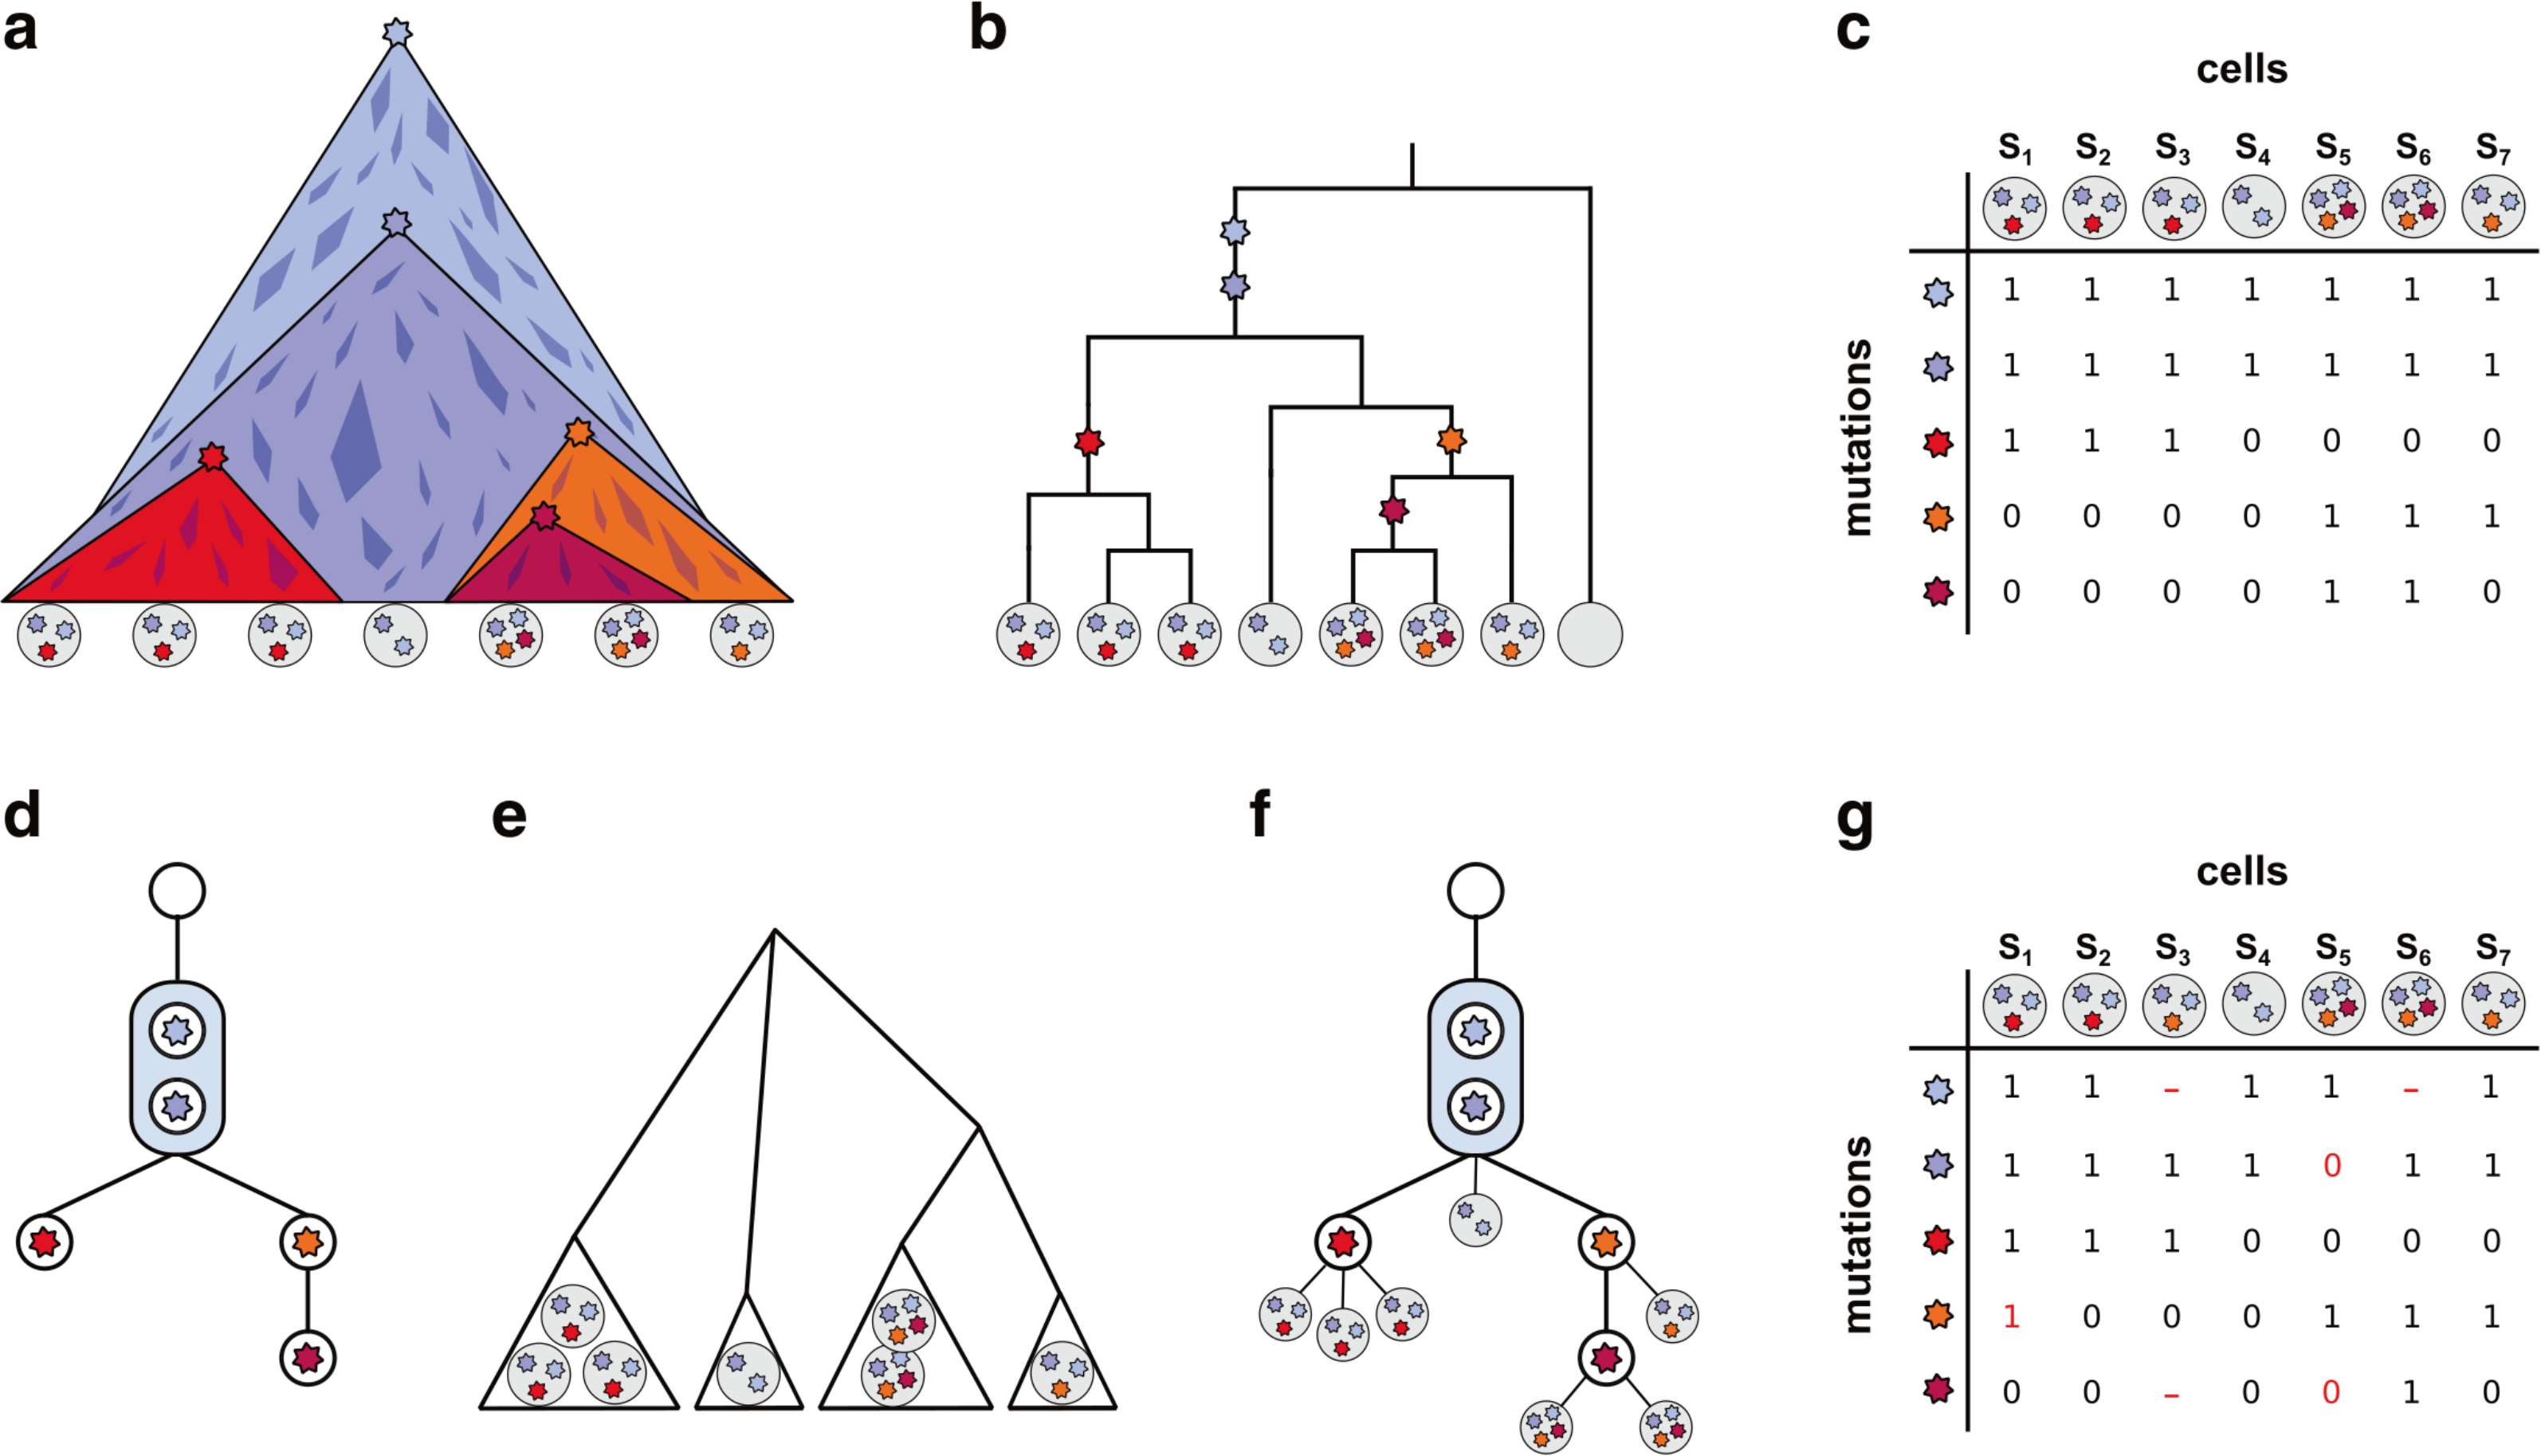
\includegraphics[width=\textwidth]{figures/example_tree.png}
    \centering
    \label{fig:example_tree}
    \caption{``Tumor evolution and cell phylogeny. \textbf{a} Schematic representation of tumor evolution with time progressing downwards. Stars denote new mutations leading to subclone expansion. The quadrangles belong to minor extinct subclones with no traces in the present-day populations. The mutations founding these clones may not have induced a sufficient growth advantage to have surviving descendant cells or may have been lost by chance. The gray discs on the bottom denote single cells sequenced after tumor removal. The stars they contain indicate the mutations observed in the cell. \textbf{b} Binary genealogical tree of the sequenced cells. An empty disc represents a normal somatic cell, which is an outgroup for the tumor cells. \textbf{c} Binary mutation matrix representing the mutation status of the sequenced tumor cells. A zero entry denotes the absence of a mutation in the respective cell, while a one denotes its presence. \textbf{d} The perfect phylogeny represented as a mutation tree, the partial (temporal) order of the mutation events. Mutations are summarized in a single node when their order is unidentifiable from the sampled cells, as is the case here for the two top-most mutations with the matrix from (c). \textbf{e} Hierarchical subclone structure. Cells with identical mutation profiles cluster into subclones, which serve as taxa in this phylogenetic tree. \textbf{f} Mutation tree with single-cell samples attached. \textbf{g} Noisy mutation matrix with missing values. The red numbers indicate flipped mutation states with respect to the true mutation matrix in (c). For 0→ 1, a false positive, the mutation is called but not present in the cell. For 1→ 0, a false negative, the mutation is not called but present in the cell, most likely due to allelic dropout during the DNA amplification. The red dash indicates a missing value; it is unknown whether the site is mutated or in the normal state in this cell.'' Copyright (C) Katharina Jahn et al., CC-BY 4.0, screenshot and cropped}
\end{figure}

\todo[inline]{Describe example tree, cell attachment, assumed true mutation matrix, concept of likelihood}

Finding a maximum-likelihood tree however is not easy. If $n$ genes are considered, the number of trees is in $O(n!)$ (Prüfer Codes), which makes an exhaustive search impractical. Jahn et al. therefore designed \ac{SCITE} as a \ac{MCMC} algorithm to empirically find the maximum likelihood tree.

\todo[inline]{Find a good paper for Prüfercodes}

A Monte Carlo algorithm runs a random experiment that produces a possible solution to a problem and evaluates how well the generated solution solves the problem. This loop of generating and evaluating a solution is then repeated multiple times and the result is the best solution the algorithm has encountered. In theory, it would suffice if the experiment had a probability greater than zero to produce a good solution, but in order to improve the solution quality and to reduce the required repetitions, one would use an experiment that produces the best solutions with a higher probability than worse solutions and that can be repeated quickly. As the name implies, \ac{MCMC} algorithms are Monte Carlo algorithms that simulate a Markov Chain to produce solutions. The advantage of using Markov Chains is that the next sample may depend on the previous one and the algorithm therefore only needs to introduce small changes to the solution. This is often faster than generating a new solution from scratch and if the current sample is already a good solution, the change may preserve some of its quality. However, a designer of a \ac{MCMC} algorithm has to make sure that the chain actually converges on the desired distribution.

\section{Goals, Results and Structure of the Thesis}

\todo[inline]{Insert the correct performance figures}

The goal for the thesis was to accelerate the SCITE algorithm with FPGAs. This new implementation, which we called \ac{ffSCITE}, should perform more chain steps per second than the initial implementation without a loss of solution quality. ffSCITE uses the Intel Stratix 10 GX 2800 FPGAs of the Noctua 2 supercomputer at the Paderborn University and executes up to XY chain steps per second, which is XY as much as SCITE executes at comparable loads. Additionally, we were also able to verify that the solutions found by \ac{SCITE} and \ac{ffSCITE} are equivalent using the \ac{TOST} \cite{schuirmann1987comparison} procedure. We had also set ourselves the optional goals to beat the optimized CPU version of \ac{SCITE} by Ernst et al. \cite{ernst2020Performance} and adapt our implementation to \ac{SCITE}'s successor \ac{infSCITE} \cite{kuipers2017single}. However, we were not able to achieve or verify this due to a lack of time.

The rest of this thesis is structured as follows: First, we will describe the original \ac{SCITE} implementation in detail, which was also the initial state of \ac{ffSCITE}. Then, we describe the final design of \ac{ffSCITE} and point out the differences to \ac{SCITE}. Some differences require more detailed descriptions and are therefore then. Lastly, we present the design and the results of the quality and performance benchmarks and list open directions that could improve \ac{ffSCITE} even further.

\todo[inline]{Update structure}